\documentclass[twoside]{book}

% Packages required by doxygen
\usepackage{fixltx2e}
\usepackage{calc}
\usepackage{doxygen}
\usepackage[export]{adjustbox} % also loads graphicx
\usepackage{graphicx}
\usepackage[utf8]{inputenc}
\usepackage{makeidx}
\usepackage{multicol}
\usepackage{multirow}
\PassOptionsToPackage{warn}{textcomp}
\usepackage{textcomp}
\usepackage[nointegrals]{wasysym}
\usepackage[table]{xcolor}

% Font selection
\usepackage[T1]{fontenc}
\usepackage[scaled=.90]{helvet}
\usepackage{courier}
\usepackage{amssymb}
\usepackage{sectsty}
\renewcommand{\familydefault}{\sfdefault}
\allsectionsfont{%
  \fontseries{bc}\selectfont%
  \color{darkgray}%
}
\renewcommand{\DoxyLabelFont}{%
  \fontseries{bc}\selectfont%
  \color{darkgray}%
}
\newcommand{\+}{\discretionary{\mbox{\scriptsize$\hookleftarrow$}}{}{}}

% Page & text layout
\usepackage{geometry}
\geometry{%
  a4paper,%
  top=2.5cm,%
  bottom=2.5cm,%
  left=2.5cm,%
  right=2.5cm%
}
\tolerance=750
\hfuzz=15pt
\hbadness=750
\setlength{\emergencystretch}{15pt}
\setlength{\parindent}{0cm}
\setlength{\parskip}{3ex plus 2ex minus 2ex}
\makeatletter
\renewcommand{\paragraph}{%
  \@startsection{paragraph}{4}{0ex}{-1.0ex}{1.0ex}{%
    \normalfont\normalsize\bfseries\SS@parafont%
  }%
}
\renewcommand{\subparagraph}{%
  \@startsection{subparagraph}{5}{0ex}{-1.0ex}{1.0ex}{%
    \normalfont\normalsize\bfseries\SS@subparafont%
  }%
}
\makeatother

% Headers & footers
\usepackage{fancyhdr}
\pagestyle{fancyplain}
\fancyhead[LE]{\fancyplain{}{\bfseries\thepage}}
\fancyhead[CE]{\fancyplain{}{}}
\fancyhead[RE]{\fancyplain{}{\bfseries\leftmark}}
\fancyhead[LO]{\fancyplain{}{\bfseries\rightmark}}
\fancyhead[CO]{\fancyplain{}{}}
\fancyhead[RO]{\fancyplain{}{\bfseries\thepage}}
\fancyfoot[LE]{\fancyplain{}{}}
\fancyfoot[CE]{\fancyplain{}{}}
\fancyfoot[RE]{\fancyplain{}{\bfseries\scriptsize Generated by Doxygen }}
\fancyfoot[LO]{\fancyplain{}{\bfseries\scriptsize Generated by Doxygen }}
\fancyfoot[CO]{\fancyplain{}{}}
\fancyfoot[RO]{\fancyplain{}{}}
\renewcommand{\footrulewidth}{0.4pt}
\renewcommand{\chaptermark}[1]{%
  \markboth{#1}{}%
}
\renewcommand{\sectionmark}[1]{%
  \markright{\thesection\ #1}%
}

% Indices & bibliography
\usepackage{natbib}
\usepackage[titles]{tocloft}
\setcounter{tocdepth}{3}
\setcounter{secnumdepth}{5}
\makeindex

% Hyperlinks (required, but should be loaded last)
\usepackage{ifpdf}
\ifpdf
  \usepackage[pdftex,pagebackref=true]{hyperref}
\else
  \usepackage[ps2pdf,pagebackref=true]{hyperref}
\fi
\hypersetup{%
  colorlinks=true,%
  linkcolor=blue,%
  citecolor=blue,%
  unicode%
}

% Custom commands
\newcommand{\clearemptydoublepage}{%
  \newpage{\pagestyle{empty}\cleardoublepage}%
}

\usepackage{caption}
\captionsetup{labelsep=space,justification=centering,font={bf},singlelinecheck=off,skip=4pt,position=top}

%===== C O N T E N T S =====

\begin{document}

% Titlepage & ToC
\hypersetup{pageanchor=false,
             bookmarksnumbered=true,
             pdfencoding=unicode
            }
\pagenumbering{alph}
\begin{titlepage}
\vspace*{7cm}
\begin{center}%
{\Large Produtor P3 \\[1ex]\large 1.\+0.\+0 }\\
\vspace*{1cm}
{\large Generated by Doxygen 1.8.14}\\
\end{center}
\end{titlepage}
\clearemptydoublepage
\pagenumbering{roman}
\tableofcontents
\clearemptydoublepage
\pagenumbering{arabic}
\hypersetup{pageanchor=true}

%--- Begin generated contents ---
\chapter{Hierarchical Index}
\section{Class Hierarchy}
This inheritance list is sorted roughly, but not completely, alphabetically\+:\begin{DoxyCompactList}
\item Q\+Main\+Window\begin{DoxyCompactList}
\item \contentsline{section}{Main\+Window}{\pageref{class_main_window}}{}
\end{DoxyCompactList}
\end{DoxyCompactList}

\chapter{Class Index}
\section{Class List}
Here are the classes, structs, unions and interfaces with brief descriptions\+:\begin{DoxyCompactList}
\item\contentsline{section}{\mbox{\hyperlink{class_main_window}{Main\+Window}} \\*Esta classe gera a janela do produtor de arquivos }{\pageref{class_main_window}}{}
\end{DoxyCompactList}

\chapter{Class Documentation}
\section{Main\+Window Class Reference}
\label{class_main_window}\index{Main\+Window@{Main\+Window}}
Inheritance diagram for Main\+Window\+:\begin{figure}[H]
\begin{center}
\leavevmode
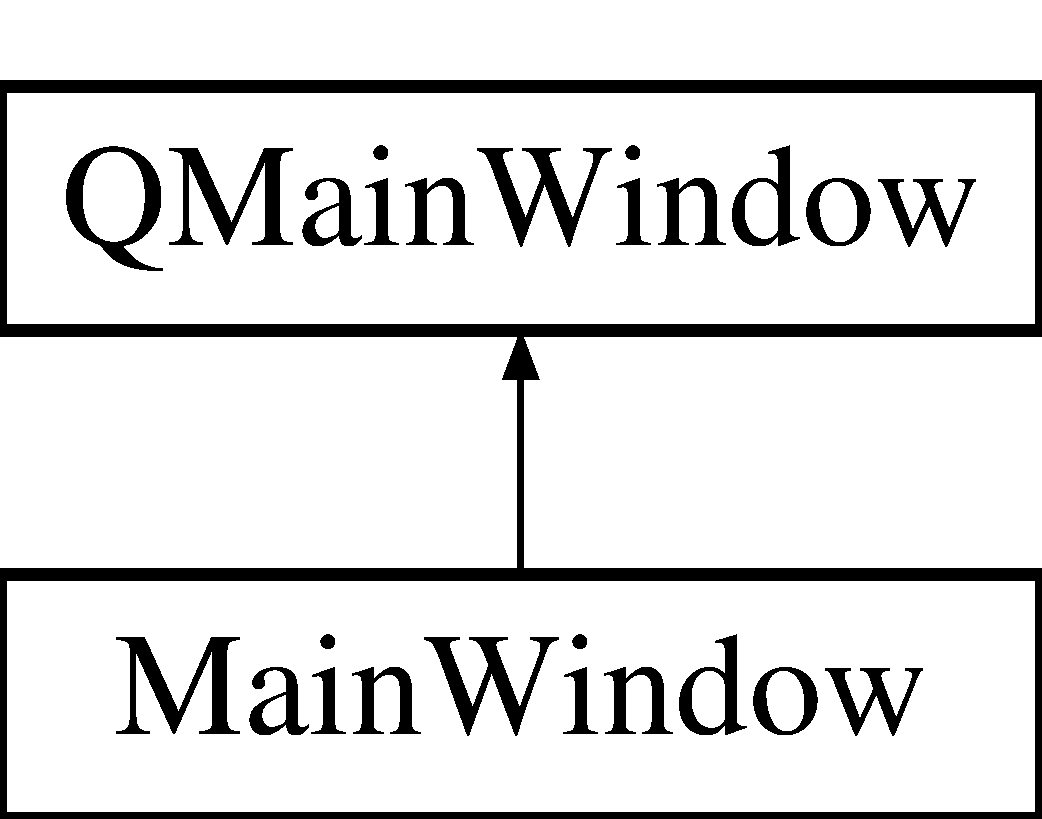
\includegraphics[height=2.000000cm]{class_main_window}
\end{center}
\end{figure}
\subsection*{Public Slots}
\begin{DoxyCompactItemize}
\item 
\mbox{\label{class_main_window_a4a2ddf4cf2ec8e240cc340416b1df792}} 
void \textbf{ get\+Data} ()
\begin{DoxyCompactList}\small\item\em Recebe os dados enviados ao servidor. \end{DoxyCompactList}\item 
\mbox{\label{class_main_window_a9d08a694a5f9c532225754381b8011ea}} 
void \textbf{ timer\+Event} (Q\+Timer\+Event $\ast$e)
\begin{DoxyCompactList}\small\item\em Manipula os eventos de tempo. \end{DoxyCompactList}\item 
\mbox{\label{class_main_window_ac5b669957c442b6eb68573dacfce33e1}} 
void \textbf{ tcp\+Connect} ()
\begin{DoxyCompactList}\small\item\em Inicia a comunicação com o servidor. \end{DoxyCompactList}\item 
\mbox{\label{class_main_window_a4d22c4c7afc7ba0a2fa4c70515c85dda}} 
void \textbf{ tcp\+Disconnect} ()
\begin{DoxyCompactList}\small\item\em Finaliza a comunicação com servidor. \end{DoxyCompactList}\item 
\mbox{\label{class_main_window_a5edcbc314e782645cdf4db101eeb247d}} 
void \textbf{ start} ()
\begin{DoxyCompactList}\small\item\em Inicia o processo de aquisição de dados. \end{DoxyCompactList}\item 
\mbox{\label{class_main_window_a939e90ddfe07d74be87b351ca2171fb0}} 
void \textbf{ stop} ()
\begin{DoxyCompactList}\small\item\em Finaliza o processo de aquisição de dados. \end{DoxyCompactList}\item 
\mbox{\label{class_main_window_a128f71880d4b9683149023fc46fcc9f8}} 
void \textbf{ update} ()
\begin{DoxyCompactList}\small\item\em Atualiza a lista de ips produtores de dados. \end{DoxyCompactList}\item 
\mbox{\label{class_main_window_a0bc5dbb811cabab53521e722fec6d966}} 
void \textbf{ update\+Line\+Edit\+IP} ()
\begin{DoxyCompactList}\small\item\em Conecta-\/se ao ip selecionado. \end{DoxyCompactList}\end{DoxyCompactItemize}
\subsection*{Public Member Functions}
\begin{DoxyCompactItemize}
\item 
\mbox{\label{class_main_window_a8b244be8b7b7db1b08de2a2acb9409db}} 
\textbf{ Main\+Window} (Q\+Widget $\ast$parent=0)
\begin{DoxyCompactList}\small\item\em Construtor da classe. \end{DoxyCompactList}\item 
\mbox{\label{class_main_window_ae98d00a93bc118200eeef9f9bba1dba7}} 
\textbf{ $\sim$\+Main\+Window} ()
\begin{DoxyCompactList}\small\item\em Destrutor da classe. \end{DoxyCompactList}\end{DoxyCompactItemize}


The documentation for this class was generated from the following files\+:\begin{DoxyCompactItemize}
\item 
mainwindow.\+h\item 
mainwindow.\+cpp\end{DoxyCompactItemize}

%--- End generated contents ---

% Index
\backmatter
\newpage
\phantomsection
\clearemptydoublepage
\addcontentsline{toc}{chapter}{Index}
\printindex

\end{document}
